\chapter{Compressori assiali}

\section{Introduzione}
I compressori assiali sono macchine relativamente recenti, si tratta di una macchina nata nel dopoguerra come componente per i gruppi turbina a gas in campo aeronautico. I primi motori aeronautici costituiti da gruppo turbogas sono stati inizialmente costruiti come compressori radiali. C'è una forte correlazione tra compressione ottenibile e rendimento, oggi qualsiasi turbogas salvo eccezioni specifiche si utilizzano compressori assiali. 

Nel diagramma in figura \ref{fig:PrestComp} è presente il rendimento del compressore in funzione della velocità specifica (che ricordiamo essere la caratteristica di macchina). Si nota che all'aumentare della velocità specifica si va verso macchine assiali, fino ad un certo punto della storia le macchine assiali non hanno goduto di rendimenti competitivi. In rosso è presentata la curva dello stato attuale dei rendimenti per macchine assiali. 
\begin{figure}
\centering
  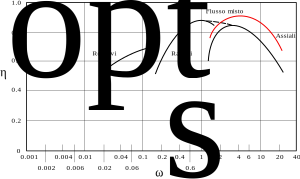
\includegraphics[width=\textwidth]{fig/PrestComp.pdf}
\caption{A destra le curve di rendimento per le macchine assiali. Si nota l'evidente aumento delle prestazioni (in rosso) rispetto alle prime macchine}
\label{fig:PrestComp}
\end{figure}
\begin{align*}
\omega_s = \cfrac{\sqrt{\phi}}{\psi^{3/4}} \cdot \sqrt{\bigg( \cfrac{D_e}{D_i} \bigg)^2 -1}
\end{align*}
\begin{align*}
\phi = \frac{Q}{u \cdot S}
\end{align*}
\begin{align*}
\psi = \cfrac{\Delta h_{0is}}{\cfrac{u^2}{2}}
\end{align*}

Nel diagramma termodinamico sono riportati gli stati 1: ingresso statore 2: uscita statore - entrata rotore 3: uscita statore. Nella parte rotorica avviene il lavoro con un relativo aumento della velocità mentre nello c'è il recupero in termini di pressione. Nello studio della macchina assiale vengono fatte generalmente le seguenti assunzioni:
\begin{itemize}
\item Flusso adiabatico;
\item Stadio "normale" o "ripetuto": tutti gli stadi hanno gli stessi profili
\begin{align*}
c_1 = c_2 \Rightarrow h_3-h_1 = h_{03} - h_{01}
\end{align*}
\item Velocità assiale costante (coincide con la velocità meridiana)
\begin{align*}
c_{m1} = c_{m2}
\end{align*}
\item densità costante nello stadio
\begin{align*}
\rho = cost. 
\end{align*}
\end{itemize}

\section{Lavoro e triangoli di velocità}
Nel rotore si conserva la rotalpia
\begin{equation}
h_1 + \frac{1}{2} \omega_1^2 = h_2 + \frac{1}{2} \omega_2^2
\end{equation}
Nello statore si conserva l'entalpia
\begin{equation}
h_2 + \frac{1}{2} c_2^2 = h_3 + \frac{1}{2} c_3^2
\end{equation}
Il lavoro scambiato è quello che avviene nella parte rotorica
\begin{equation}
\lambda = \frac{u \cdot c_{u2} - u \cdot c_{u1}}{u^2} = \frac{c_{u2} - c_{u1}}{u}
\end{equation}

Posso quindi andare a disegnare i triangoli di velocità relativi allo stadio elementare. La componente meridiana e periferica sono costanti. Posso scrivere le relazioni che legano gli angoli con le velocità in uscita. 
\begin{align*}
c_{u2} = u - \omega_{u2}
\end{align*}
\begin{align*}
\omega_{u2} = c_m \tan \beta_2
\end{align*}
\begin{align*}
c_{u1} = c_m \tan \alpha_1
\end{align*}
Posso quindi scrivere
\begin{align*}
\lambda = 1- \frac{\omega_{u2}}{u} - \frac{c_{u1}}{u} = 1 - \frac{c_m}{u} \left(\tan \beta_2 + \tan \alpha_1 \right)
\end{align*}
Ma definendo 
\begin{align*}
\Phi = \frac{c_m}{u}
\end{align*}
\begin{equation}
\lambda = 1 - \Phi \left( \tan \beta_2 + \tan \alpha_1 \right) = 1 - k \cdot \Phi
\end{equation}
Con $k$ costante che dipende dalla geometria della macchina. Si tratta di una rappresentazione molto simile a quella nel caso delle pompe centrifuche nelle quali a sedona del valore di $k$ si ha la curva caratteristica della pompa; questo viene chiarito meglio dal diagramma in figura \ref{fig:CondProg}.
\begin{figure}
\centering
  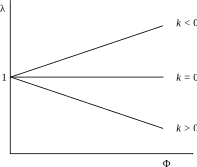
\includegraphics[width=.4\textwidth]{fig/CondProg.pdf}
\caption{}
\label{fig:CondProg}
\end{figure}
Andiamo ora a definire una condizione particolare di progetto "lambda design" $\lambda_d$.
\begin{align*}
\lambda_d = 1 - k \cdot \Phi_d, \;\; k = f(\lambda_d,\Phi_d)
\end{align*}
Calcolo ora il rapporto $\lambda/\lambda_d$:
\begin{equation} \label{eq:lambdad}
\frac{\lambda}{\lambda_d} = \frac{1}{\lambda_d} - \frac{\Phi}{\Phi_d} \Bigg( \frac{1-\lambda_d}{\lambda_d}, \;\;\; 0.3 < \lambda_d < 0.4
\end{equation}
In figura \ref{fig:LambdaPhiChart} è rappresentato il diagramma caratteristico però in termini di rapporti rispetto alle condizioni di progetto. Si vede che nel caso ideale di $\lambda_d = 1$ il lavoro scambiato sarebbe indipendente dalla portata, sarebbe una situazione abbastanza attraente. 
\begin{figure}
\centering
\begin{minipage}{.5\textwidth}
  \centering
  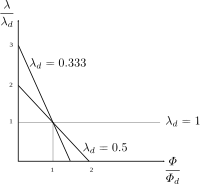
\includegraphics[width=.9\linewidth]{fig/LambdaPhiChart.pdf}
  \captionof{figure}{}
  \label{fig:LambdaPhiChart}
\end{minipage}%
\begin{minipage}{.5\textwidth}
  \centering
  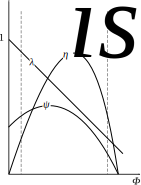
\includegraphics[width=.9\linewidth]{fig/CarattReal.pdf}
  \captionof{figure}{}
  \label{fig:CarattReal}
\end{minipage}
\end{figure}
Generalmente in un compressore, infatti, la pressione di output è definita mentre la portata è regolata, $\lambda_d = 1$ avrei una macchina perfetta, il rapporto di pressione lo riuscirei sempre a mantenere e basta che regoli la portata per ottenere la pressione voluta. Purtroppo non è così perchè le palettature non si comportano in modo ideale, si hanno separazioni di vela, inspessimenti di strato limite... dal punto di vista realistico si riesce ad ottenere un $\lambda_d$ definito come nell'equazione \ref{eq:lambdad}. 

Come mostrato in figura \ref{fig:CarattReal} otterrò un comportamento non ideale che non avrà andament rettilineo, avrtò quindi un campo di utilizzo essendo limitato sia a portate basse che a portate alte. 

Caratteristica reale:
\begin{equation}
\psi = \frac{\Delta h_{0is}}{u^2} = \lambda \cdot \eta_{is}, \;\;\; \Delta h_{0is} = h_{30is} - h_{10}
\end{equation}

Non abbiamo ancora detto nulla riguardo la forma della pala in funzione del grado di reazione (salto elaborato tra parte statorica e parte rotorica). Vado a sviluppare il grado di reazione della macchina:
\begin{equation}
R = \frac{h_2 - h_1}{h_3-h_1} 
\end{equation}
\begin{align*}
R = \frac{\omega_1^2 - \omega_2^2}{2 u (c_{u2} - c_{u1})} = \frac{(\omega_{u1} + \omega_{u2})(\omega_{u1}-\omega_{u2})}{2 u (c_{u2} - c_{u1})}
\end{align*}
\begin{align*}
\begin{rcases*}
c_{u2} = u - \omega_{u2}\\
c_{u1} = u - \omega_{u1}
\end{rcases*}
\Rightarrow c_{u2} - c_{u1} = \omega_{u1} - \omega_{u2} 
\end{align*}
Definendo poi
\begin{align*}
\tan \beta_{\infty} = \frac{\tan \beta_1 + \tan \beta_2}{2}, \;\; \Phi = \frac{c_m}{u}
\end{align*}
Si ottiene
\begin{equation}
\boxed{R = \Phi \tan \beta_{\infty} = \frac{\omega_{u \infty}}{u}}
\end{equation}
Lo stesso risultato poteva essere raggiunto nel seguente modo
\begin{equation}
\omega_u1 = u - c_{u1} \; \Rightarrow \; R = \frac{1}{2} + \frac{\tan \beta_2 - \tan \alpha_1}{2} \cdot \Phi \simeq \frac{1}{2} + \cos \Phi
\end{equation}
Quello che è importante notare è che:
\begin{align*}
R = 0.5 \to \beta_2 = \alpha_1
\end{align*}
Il grado di reazione è costante con la portata e la palettatura sarà simmetrica.

Per rappresentare lo stadio al variare del grado di reazione andiamo per prima cosa a definire i triangoli di velocità come si vede in figura INSERISCI FIGURA.
\begin{figure}
\centering
  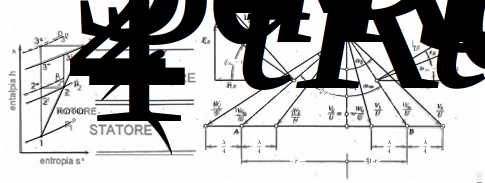
\includegraphics[width=\textwidth]{fig/StadioRipetuto.pdf}
\caption{}
\label{fig:StadioRipetuto}
\end{figure}
Posso quindi scrivere
\begin{align*}
r \cdot \tan \beta_{\infty} = R 
\end{align*}
\begin{align*}
\lambda = \cfrac{\Delta h_0}{\cfrac{u^2}{2}} = \cfrac{u \Delta c_u}{\cfrac{u^2}{2}} = \cfrac{2 \Delta c_u}{u} = \cfrac{2 \Delta \omega_u}{u}
\end{align*}
\begin{align*}
\frac{\Delta c_u}{u} = \frac{\Delta \omega_u}{u} = \frac{\lambda}{2}
\end{align*}
Qual'ora si operi un cambio di portata vediamo che i triangoli di velocità non cambiano, quello che cambia è la cifra di flusso che passa da phi design a phi come si vede in figura \ref{fig:CondFuoriProg}.
\begin{figure}
\centering
  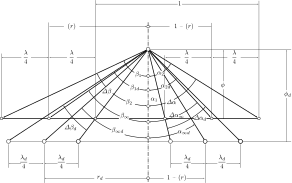
\includegraphics[width=\textwidth]{fig/CondFuoriProg.pdf}
\caption{}
\label{fig:CondFuoriProg}
\end{figure}
Possiamo classificare alcune condizioni notevoli riportate in figura .
\begin{figure}
\centering
  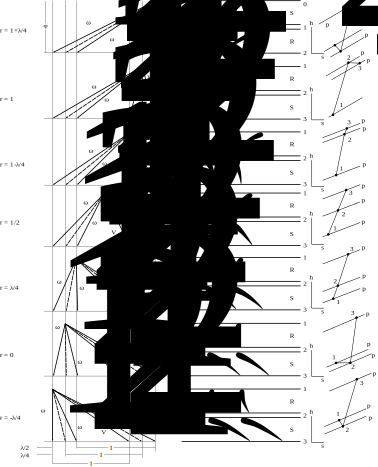
\includegraphics[width=1.3\textwidth]{fig/ComprAssTab.pdf}
\caption{}
\label{fig:ComprAssTab}
\end{figure}
Il primo caso con $r = 1 + \lambda /4$ è particolare in quanto si ha grado di reazione maggiore di uno, lo statore precede infatti il rotore. Mi ritrovo con una velocità di uscita puramente assiale.

Con grado di reazione $r = 1$ le velocità assolute ingresso uscita sono simmetriche.

Con $r = 1 - \lambda/4$ la velocità assoluta è puramente assiale, mentre quella lallo scarico non lo è. 

Sono poi rappresentate le geometrie per gradi di reazione sempre più ridotti. 

La soluzione $r = 1/2$ è la più diffusa e utilizzata eccetto per il primo e l'ultimo stadio in cui si vogliono distribuzioni di velocità particolari, velicità assoluta in uscita e poi in ingresso puramente assiale. In questa configurazione si avranno profili uguali ma specchiati, l'intervallo p1 p3 è poi diviso equamente in due parti uguali tra la parte statorica e la parte rotorica. 

\section{Termodinamica}
Vediamo il calcolo del rendimento al variare della portata e del grado di reazione. Partiamo dalla definizione di rendimento isoentropico
\begin{align*}
\eta = \frac{\Delta h_{is}}{\Delta h_0} = \frac{\Delta p}{\rho \cdot \Delta h_0}
\end{align*}
Dal primo principio:
\begin{align*}
T ds = dh - \frac{dp}{\rho}
\end{align*}
ma
\begin{align*}
ds = 0 \Rightarrow dh = \frac{dp}{\rho}
\end{align*}
Otteniamo quindi
\begin{align*}
\eta_{is} = \frac{\Delta p}{\rho \cdot \Delta h_0} = \cfrac{\Delta p}{\rho \cdot \cfrac{\lambda}{2} u^2}
\end{align*}
L'incremento di pressione totale si può però ulteriormente sviluppare come somma di incremento di pressione sviluppato nel rotore e nello statore
\begin{align*}
\Delta p = \Delta p_R + \Delta p_S = \frac{F_{aR}}{s_R} + \frac{F_{aS}}{s_S} = \frac{F_{tR} \cdot \tan(\beta_{\infty} - \varepsilon_R}{s_R} + \frac{F_{tS} \cdot \tan(\alpha_{\infty} - \varepsilon_S}{s_S}
\end{align*}
Con $\varepsilon_S, \; \varepsilon_R$ indice di efficienza del profilo
Possiamo fare qualche assunzione. I profili hanno drag molto più piccolo del lift quindi
\begin{align*}
\tan \varepsilon_R \simeq \varepsilon_R = \frac{D_R}{L_R} \;\;\; \tan \varepsilon_S \simeq \varepsilon_S = \frac{D_S}{L_S}
\end{align*}
Utilizzando le componenti di forza del triangolo di velocità si ottiene
\begin{align*}
F_{tR} = \dot{m} \Delta \omega_u = \overbrace{s_R \cdot \rho \cdot c_m}^\text{$ \dot{m} $} \cdot \overbrace{\lambda \cdot u \cdot \frac{1}{2}}^\text{$\Delta \omega_u$}  
\end{align*}

Analogamente riesco a fare la stessa cosa per la parte statorica

formule

Andando a sostituire in delta p 

formula

Ricordando le relazioni

formule

Ottengo in fine la relazione del salto di pressione in funzione del grado di reazione e di $lambda$:

equazione

Posso dire che epsilon r è circa epsilon s. Il rendimento isoentropico ricordando l'equazione RIFERIMENTO diviene:

formula rendimento

ferivando rispetto a R ottengo che

formule

Naturalmente si vede che il rendimento del compressore è migliorato alla diminuzione di epsilon

Determino ora il rendimento ottimale in funzione di phi

formule

Quindi

formule

Rappresentando l'ultima equazione ottengo 



